\chapter{Plataforma de desarrollo}
\label{cap:capitulo3}

\begin{flushright}
\begin{minipage}[]{10cm}
\emph{Cualquier cosa que pueda ser automatizada, será automatizada..}\\
\end{minipage}\\

Robert Cannon\\
\end{flushright}

\vspace{1cm}

En este capítulo se detallan los recursos hardware y software empleados para llevar a cabo el desarrollo de la aplicación. A nivel hardware, se han utilizado dos estaciones didácticas de automatización industrial del fabricante FESTO, cada una equipada con un PLC. Además, el sistema completo incluye una interfaz HMI de SIEMENS y un brazo robótico colaborativo de la empresa Universal Robots (UR). En cuanto al software, se han utilizado distintos entornos de desarrollo específicos para cada dispositivo: el software TIA Portal para la programación de los PLCs y la configuración de la HMI, y la plataforma URSim para la simulación y control del brazo robótico. Además, se han empleado librerías propias de los fabricantes, sistemas operativos compatibles con las herramientas utilizadas y conexiones mediante protocolos estándar de comunicación industrial como Profinet. También se ha realizado el montaje completo y el conexionado de todos los elementos.

\section{Estación distribución}
\label{sec:estacion_distribucion}

La estación de distribución con cinta transportadora de Festo Didactic \footnote{Image retrieved from Festo.com. (N.d.). Retrieved June 4, 2025, from \url{https://www.festo.com/es/es/p/estacion-de-distribucion-id_PROD_DID_8034566/}} es un módulo del sistema MPS (Modular Production System) que simula una parte de una línea de producción automatizada. Su función principal es clasificar, alinear y transportar piezas de trabajo desde un punto de alimentación hacia otras estaciones del sistema \cite{estacion_distribucion}. Este sistema está diseñado para la formación técnica en automatización industrial, permitiendo a estudiantes aprender a manejar sensores, actuadores, sistemas neumáticos, cintas transportadoras y PLCs. \\

\begin{figure} [h!]
  \begin{center}
    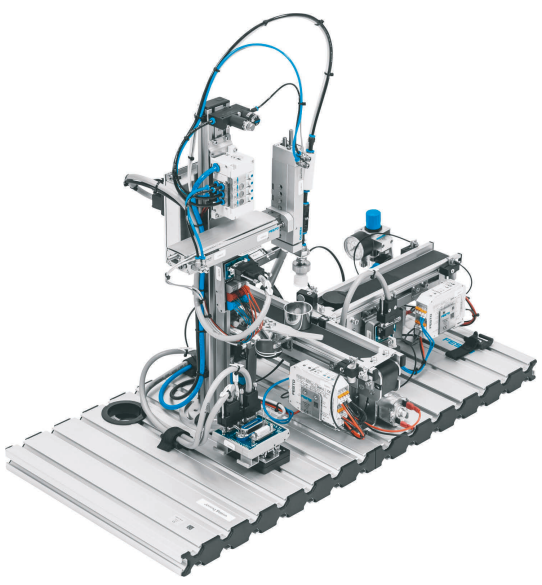
\includegraphics[width=12.5cm]{figs/estacion_distribucion_1}
  \end{center}
  \caption{\centering Estación distribución. \cite{estacion_distribucion}}
  \label{fig:estacion_distribucion_1}
\end{figure} 

En la tabla \ref{fig:estacion_distribucion_3} se detallan las características generales del sistema:

\begin{figure} [h!]
  \begin{center}
    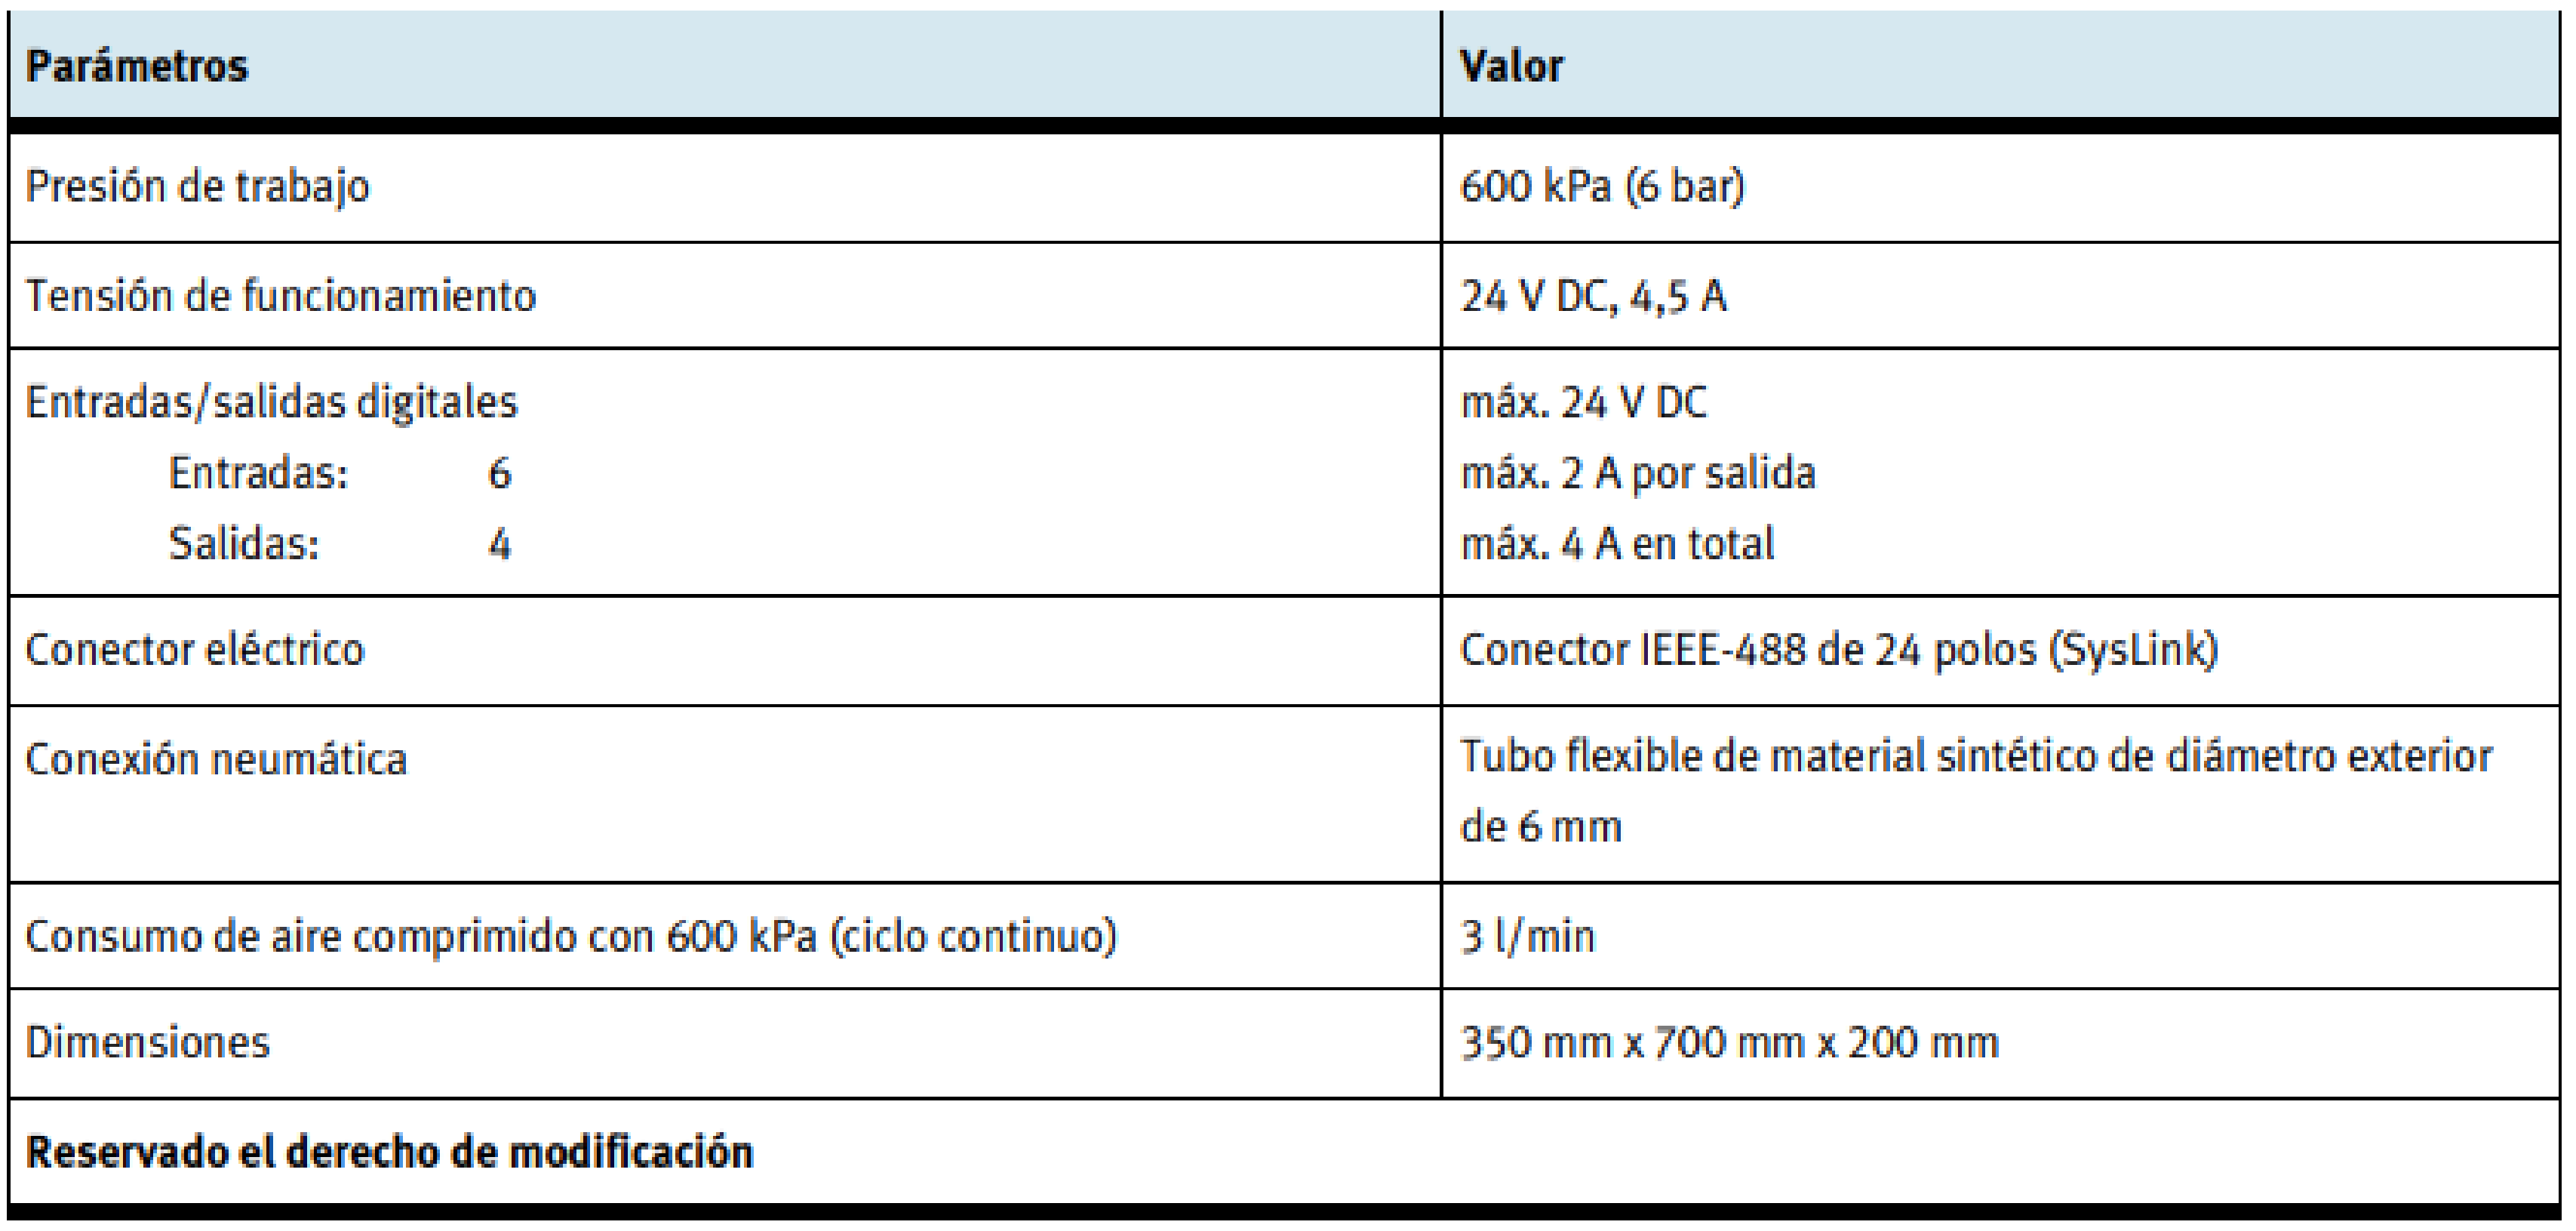
\includegraphics[width=15cm]{figs/estacion_distribucion_3}
  \end{center}
  \caption{\centering Características generales de la etación distribución. \cite{estacion_distribucion}}
  \label{fig:estacion_distribucion_3}
\end{figure} 

\clearpage

Las piezas utilizadas en las estaciones MPS de Festo Didactic están divididas en tres colores: rosa, negro y metálico. Estas piezas representan distintos tipos de materiales o componentes, lo que permite que los sensores (como óptico o inductivo) las distingan fácilmente facilitando su clasificación, inspección o tratamiento diferenciado por el sistema automatizado. Cada pieza mantiene dimensiones normalizadas para un manejo preciso y repetible y vienen equipadas con una tapa la cual puede ser colocada en estas para ofrecer mayor libertad al crear el proceso automático \\

La estación distribución está formada por los siguientes componentes:

\begin{itemize}
   \item \textbf{Almacén de piezas:} Sistema de alimentación que permite introducir piezas de trabajo de manera ordenada a mitad de la cinta transportadora. Funciona como un cargador vertical donde las piezas se apilan y se liberan una a una mediante un actuador neumático (máximo 7 piezas) \cite{estacion_distribucion}. Está diseñado para asegurar una alimentación controlada y repetible en los procesos de automatización \cite{estacion_distribucion}.
   
    \item \textbf{Cinta transportadora:} Encargada de desplazar las piezas entre las estaciones. Puede moverse en ambas direcciones. 
    
     \item \textbf{Separador:} Actuador neumático situada al inicio de la cinta cuya función es controlar el flujo de piezas en la cinta transportadora. Si se activa, retiene las piezas provenientes del inicio de la cinta y da paso a las almacenadas en el almacén de piezas \cite{estacion_distribucion}.
     
      \item \textbf{Sensor para la distinción de piezas:} El sistema viene equipado con un módulo extra situado a la mitad de la cinta el cual es capaz de distinguir el color y material de la pieza. Este sensor distingue entre tres tipos de piezas dependiendo de cuantos bits se activen. Cada bit que se activa es la salida de un sensor, el primerio es un sensor óptico que detecta presencia y se activa siempre (pieza negra), el segundo es òptico también y se enciende si la pieza rebota luz de color (pieza rosa) y el tercero es un sensor inductivo el cual se activa si la pieza es metálica. \cite{estacion_distribucion}.

    \item \textbf{Sensores láser:} La estación posee sensores ópticos y de proximidad que detectan la presencia de las piezas, funcionan mediante un láser el cual le proporciona datos al PLC.

    \item \textbf{Estructura mecánica modular:} Bastidor de perfiles de aluminio que soporta todos los componentes y permite su integración con otras estaciones del sistema MPS \cite{estacion_distribucion}.
\end{itemize}

A continuación, se muestra una imagen en la que se observan todos los componentes:

\begin{figure} [h!]
  \begin{center}
    \includegraphics[width=15cm]{figs/estacion_distribucion_2}
  \end{center}
  \caption{\centering Componentes de la estación distribución.}
  \label{fig:estacion_distribucion_2}
\end{figure} 

\section{Estación unión}
\label{sec:estacion_union}

La estación de unión de Festo Didactic\footnote{Image retrieved Festo.com.  (N.d.). Retrieved June 4, 2025, from  \url{https://www.festo.com/es/es/p/estacion-de-union-id_PROD_DID_8063910/}} simula un proceso industrial en el que se unen dos piezas mediante un actuador neumático equipado con una ventosa (Pick\&Place) \cite{estacion_union}. El objetivo de esta estación es colocerle o retirerle las tapas a las piezas que estén correctamente orientadas y así terminar la secuencia. La estación está compuesta por un brazo neumático, dos cintas para mover las piezas y tapas, sensores que detectan su presencia y adicionalmente un sensor cuya función es detectar la orientación de las piezas \cite{estacion_union}. Esta estación permite realizar prácticas de automatización como control secuencial, posicionamiento y verificación del montaje. Es ideal para formación técnica en tareas típicas de ensamblaje automatizadas. Se adjuntan las características generales de la estación como se puede ver en el gráfico \ref{fig:estacion_union_3}:


\begin{figure} [h!]
  \begin{center}
    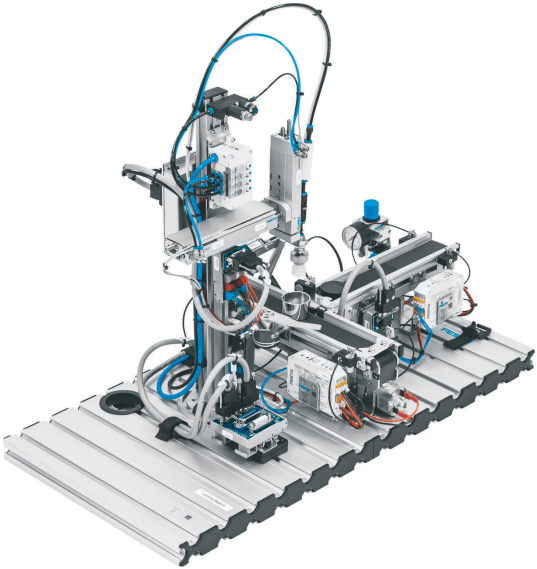
\includegraphics[width=9.75cm]{figs/estacion_union_1}
  \end{center}
  \caption{\centering Estación unión. \cite{estacion_union}}
  \label{fig:estacion_union_1}
\end{figure} 

\begin{figure} [h!]
  \begin{center}
    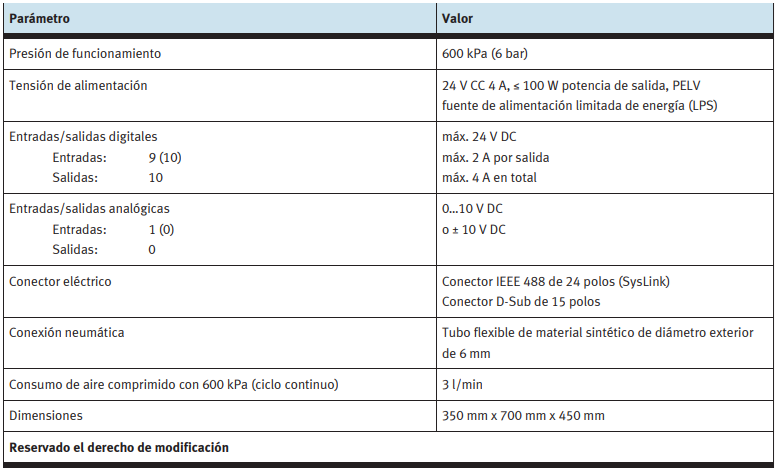
\includegraphics[width=14.5cm]{figs/estacion_union_3}
  \end{center}
  \caption{\centering Características generales de la estación unión. \cite{estacion_union}}
  \label{fig:estacion_union_3}
\end{figure} 

La estación unión está compuesta principalmente por tres módulos:

\begin{itemize}

	 \item El Módulo de \textbf{Cinta Transportadora 1} transporta, separa y acumula piezas de hasta 40 mm de diámetro. Está impulsado por un motor de corriente continua con control de velocidad y dirección, y utiliza sensores ópticos para detectar la presencia de piezas al inicio, medio y al final de la cinta \cite{estacion_union}. Un electroimán que actúa como retenedor permite detener y liberar piezas individualmente a la altura del brazo, y un sensor difuso con salida digital y analógica identifica la orientación de las piezas el cual se ayuda de un retenedor para poder hacerlo correctamente sin que se mueva la pieza \cite{estacion_union}.

	 \item El Módulo de \textbf{Cinta Transportadora 2} tiene funciones similares, pero está diseñado para manejar tanto cuerpos de piezas como tapas. También utiliza un motor de corriente continua y sensores ópticos para controlar el flujo de materiales \cite{estacion_union}.

	 \item El Módulo \textbf{Pick\&Place} es un manipulador de dos ejes que utiliza carros deslizantes de precisión y sensores de proximidad para detectar las posiciones finales. La fuerza del eje vertical puede ajustarse mediante un regulador de presión con una ventosa de fuelle y cuenta con un filtro de vacío y un presostato para asegurar una sujeción fiable \cite{estacion_union}.
\end{itemize}

\begin{figure} [h!]
  \begin{center}
    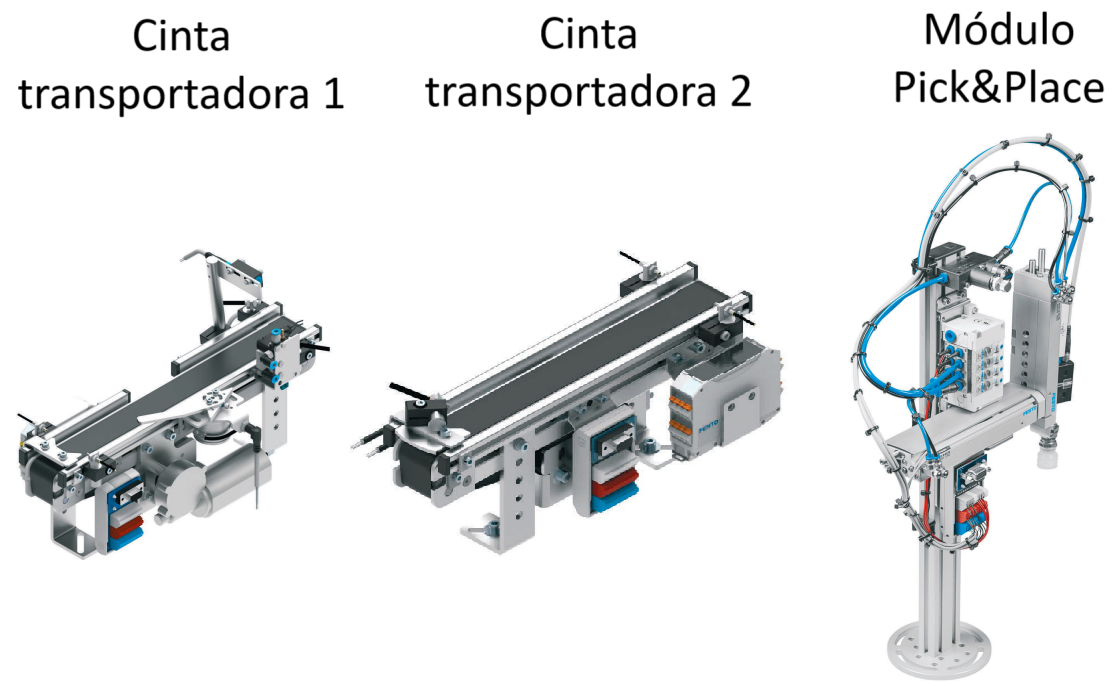
\includegraphics[width=14cm]{figs/estacion_union_2}
  \end{center}
  \caption{\centering Componentes de la estación unión. \cite{estacion_union}}
  \label{fig:estacion_union_2}
\end{figure} 

\begin{figure} [h!]
  \begin{center}
    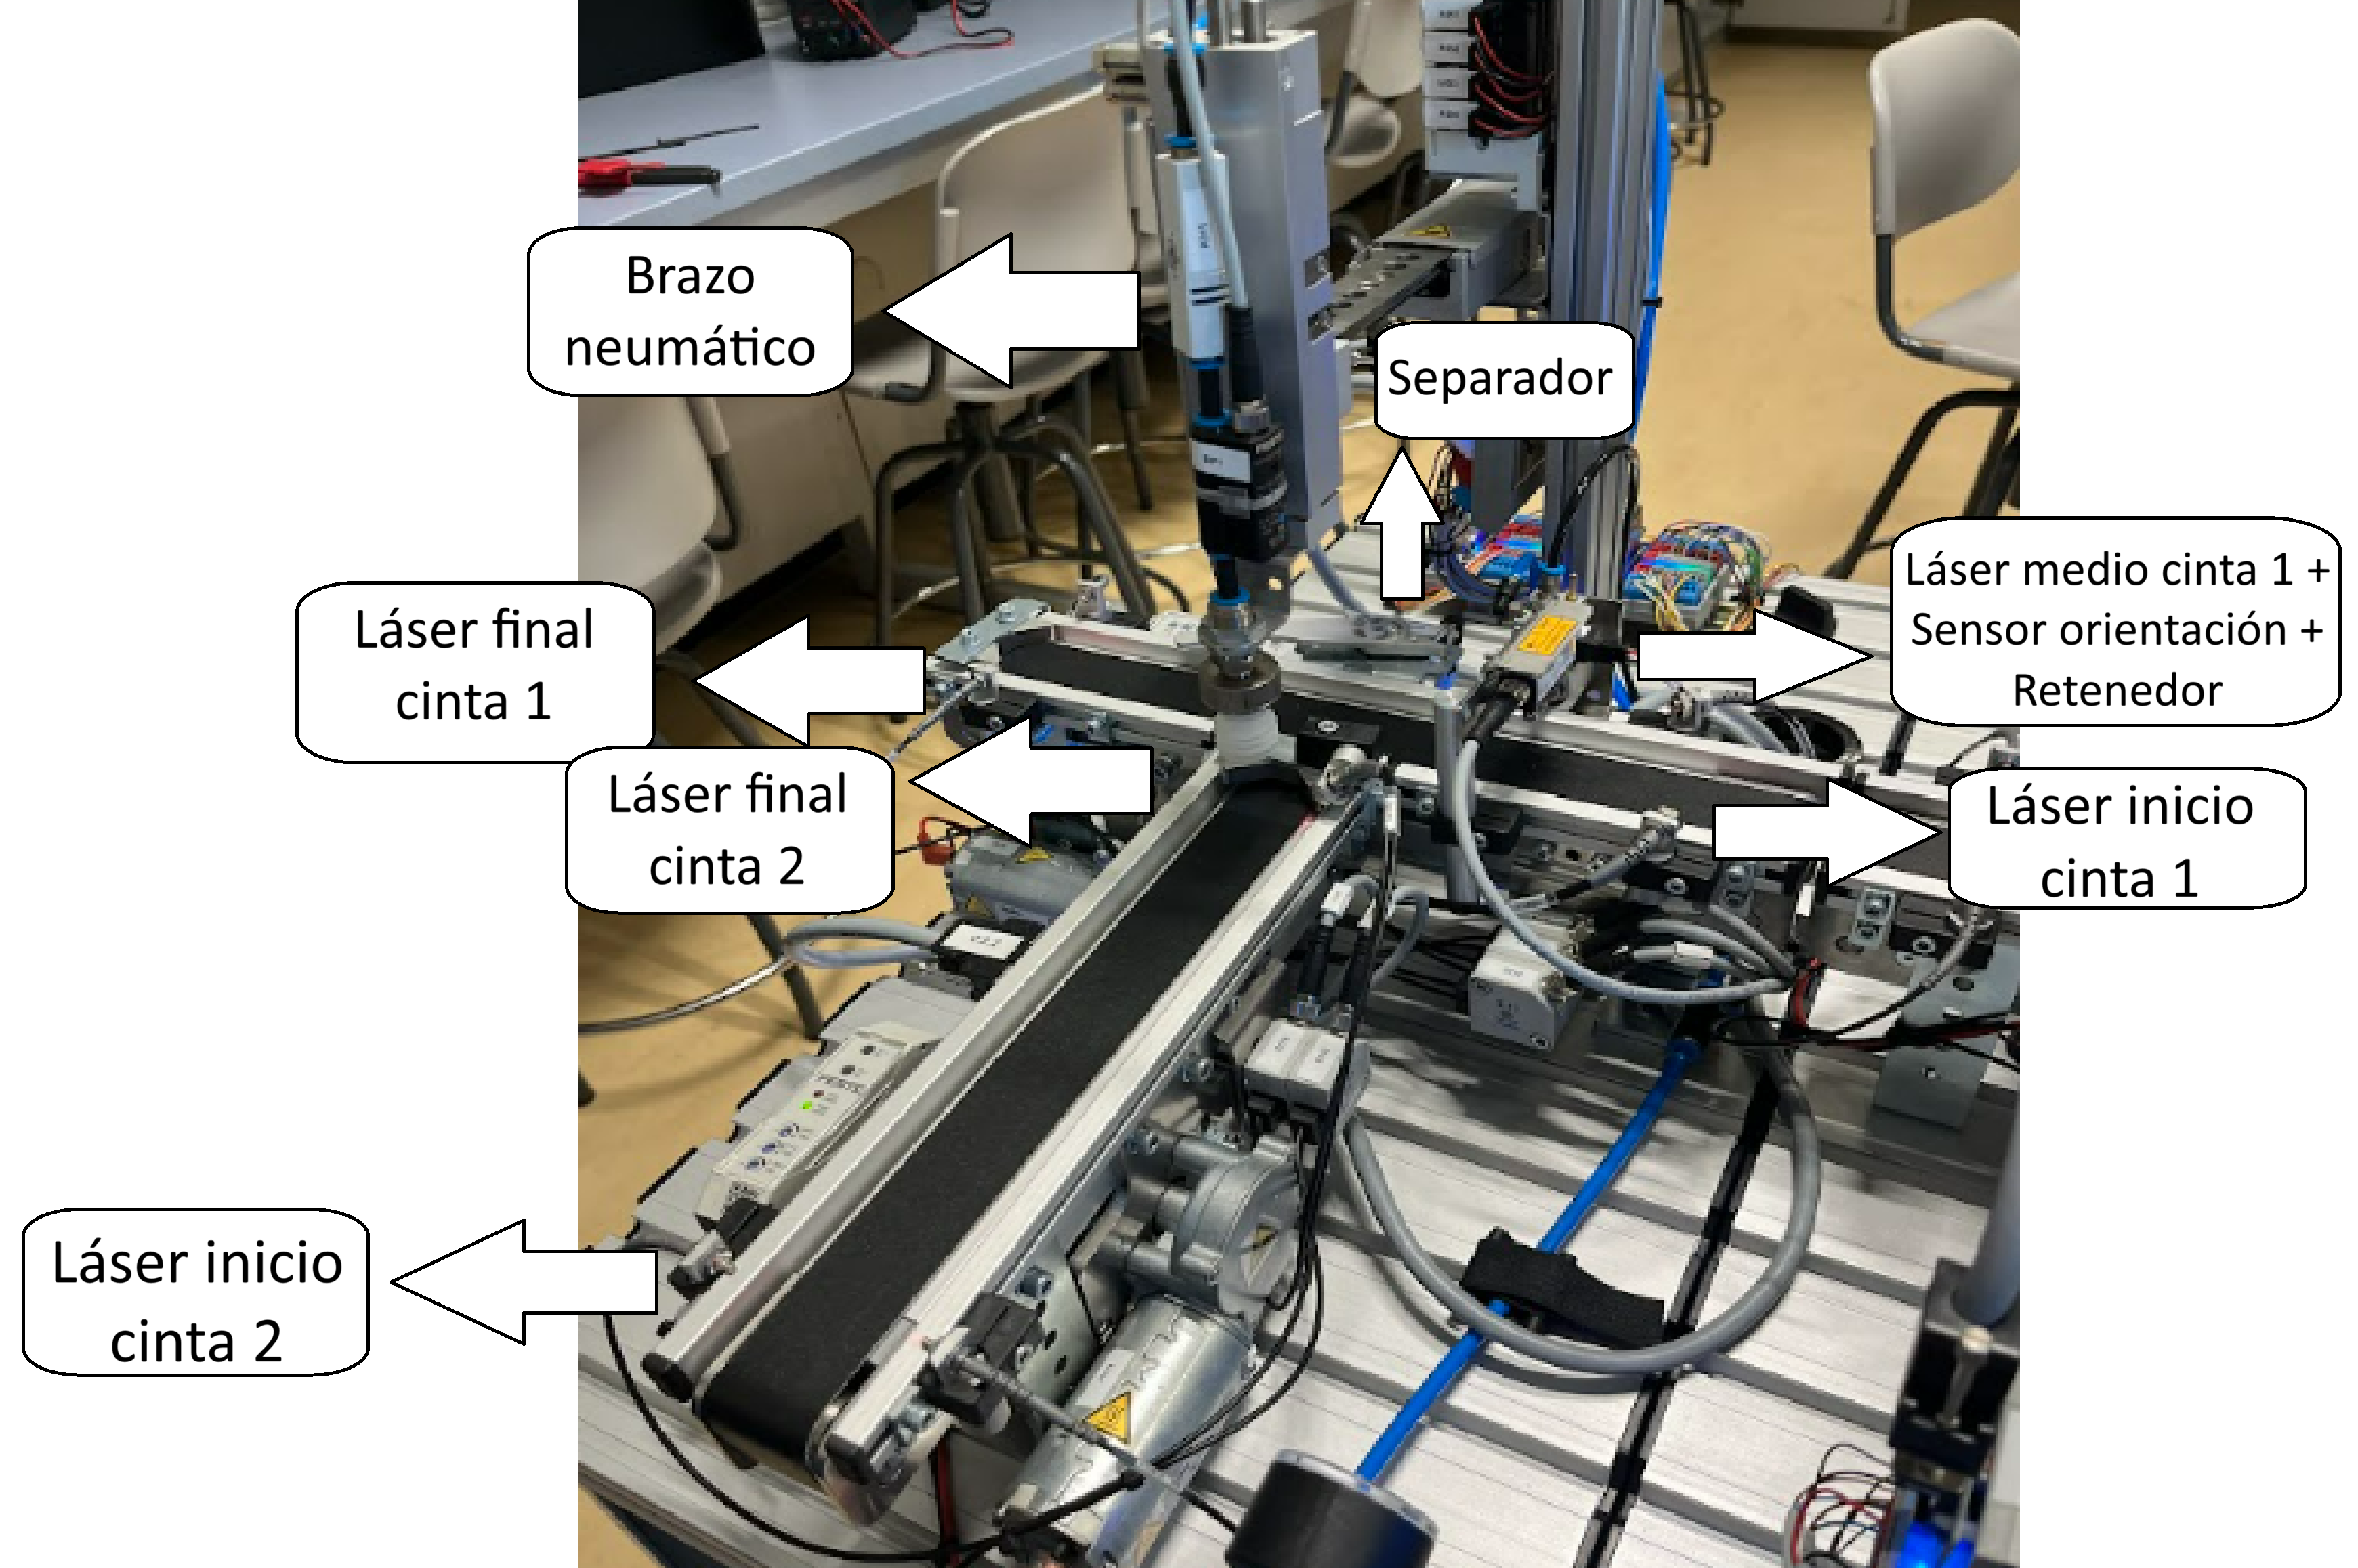
\includegraphics[width=16.5cm]{figs/estacion_union_4}
  \end{center}
  \caption{\centering Componentes de la estación unión.}
  \label{fig:estacion_union_4}
\end{figure} 

\section{PLCs Siemens 1200s}
\label{sec:plc}

Para la elaboración de este trabajo se ha utilizado el PLC Siemens S7-1200, concretamente el modelo \textbf{6ES7 215-1BG40-0XB0}. Este modelo forma parte de la familia de controladores compactos de Siemens, ampliamente utilizados en aplicaciones de automatización industrial. El PLC corresponde a la CPU 1215C con alimentación AC/DC y salidas a relé, lo que le otorga una gran versatilidad para controlar y supervisar sistemas de pequeña y mediana escala \cite{PLC_siemens}.

Entre sus características más destacadas se encuentran sus 14 entradas digitales de 24 V DC, 10 salidas digitales tipo relé de 2 A, 2 entradas analógicas (0–10 V DC) y 2 salidas analógicas (0–20 mA DC) \cite{PLC_siemens}. Esta combinación de entradas y salidas permite conectar una gran variedad de sensores y actuadores directamente al PLC sin necesidad de módulos adicionales, y además, su módulo de E/S es compatible eléctricamente con las E/S de las estaciones.

En términos de comunicación, esta CPU incorpora dos puertos PROFINET con función de switch integrado, lo que facilita su integración en redes industriales y la comunicación con dispositivos HMI, otros PLCs o sistemas SCADA \cite{PLC_siemens}. Además, es compatible con protocolos de comunicación abiertos como TCP/IP, ISO-on-TCP, UDP y MODBUS, y permite el uso de servidor OPC UA mediante licencia, una característica clave para entornos de Industria 4.0 \cite{PLC_siemens}.

\begin{figure} [h!]
  \begin{center}
    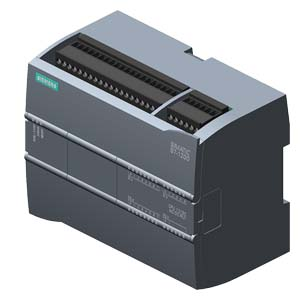
\includegraphics[width=8cm]{figs/PLC_siemens}
  \end{center}
  \caption{\centering PLC Siemens 1215 AC/DC/RLY. \cite{PLC_siemens}}
  \label{fig:PLC_siemens}
\end{figure} 

Su programación se realiza a través del software \textbf{STEP 7 (TIA Portal)} versión V20 o superior, ofreciendo compatibilidad con lenguajes como KOP (diagrama de contactos), FUP (diagrama de funciones) y SCL (lenguaje estructurado) \cite{PLC_siemens}. También dispone de funciones tecnológicas avanzadas como control PID, contadores de alta velocidad (hasta 100 kHz), y posicionamiento, lo cual amplía sus capacidades para aplicaciones más exigentes \cite{PLC_siemens}.

En cuanto a su hardware, presenta una memoria de trabajo de 200 kB y una memoria de carga de 4 MB, además de la posibilidad de insertar una tarjeta SIMATIC Memory Card para ampliar almacenamiento o realizar copias de seguridad \cite{PLC_siemens}. El diseño compacto (130 × 100 × 75 mm) y el grado de protección IP20 lo hacen ideal para entornos industriales controlados.

\section{HMI}
\label{sec:hmi}

El HMI utilizado para este proyecto es el \textbf{SIMATIC HMI KTP700 Basic PN}. Este es un panel HMI de la segunda generación de Basic Panels de Siemens, diseñado para ofrecer una interfaz hombre-máquina eficiente, compacta y rentable en tareas de visualización y operación dentro de entornos industriales. Este modelo cuenta con una pantalla táctil de 7 pulgadas, con una resolución de 800 × 480 píxeles (WVGA) y una profundidad de color de 64.000 colores, lo que proporciona una visualización clara, detallada y moderna de los procesos industriales \cite{HMI_KTP}.

Una de sus principales ventajas es la combinación de pantalla táctil y teclas de función (8 teclas de función programables), lo cual permite al operador interactuar de forma rápida e intuitiva con el sistema, incluso con guantes o en entornos con condiciones difíciles. El panel también está equipado con una interfaz PROFINET integrada, lo que lo hace ideal para la comunicación directa con controladores SIMATIC S7-1200 y otros dispositivos de automatización compatibles \cite{HMI_KTP}.

\begin{figure} [h!]
  \begin{center}
    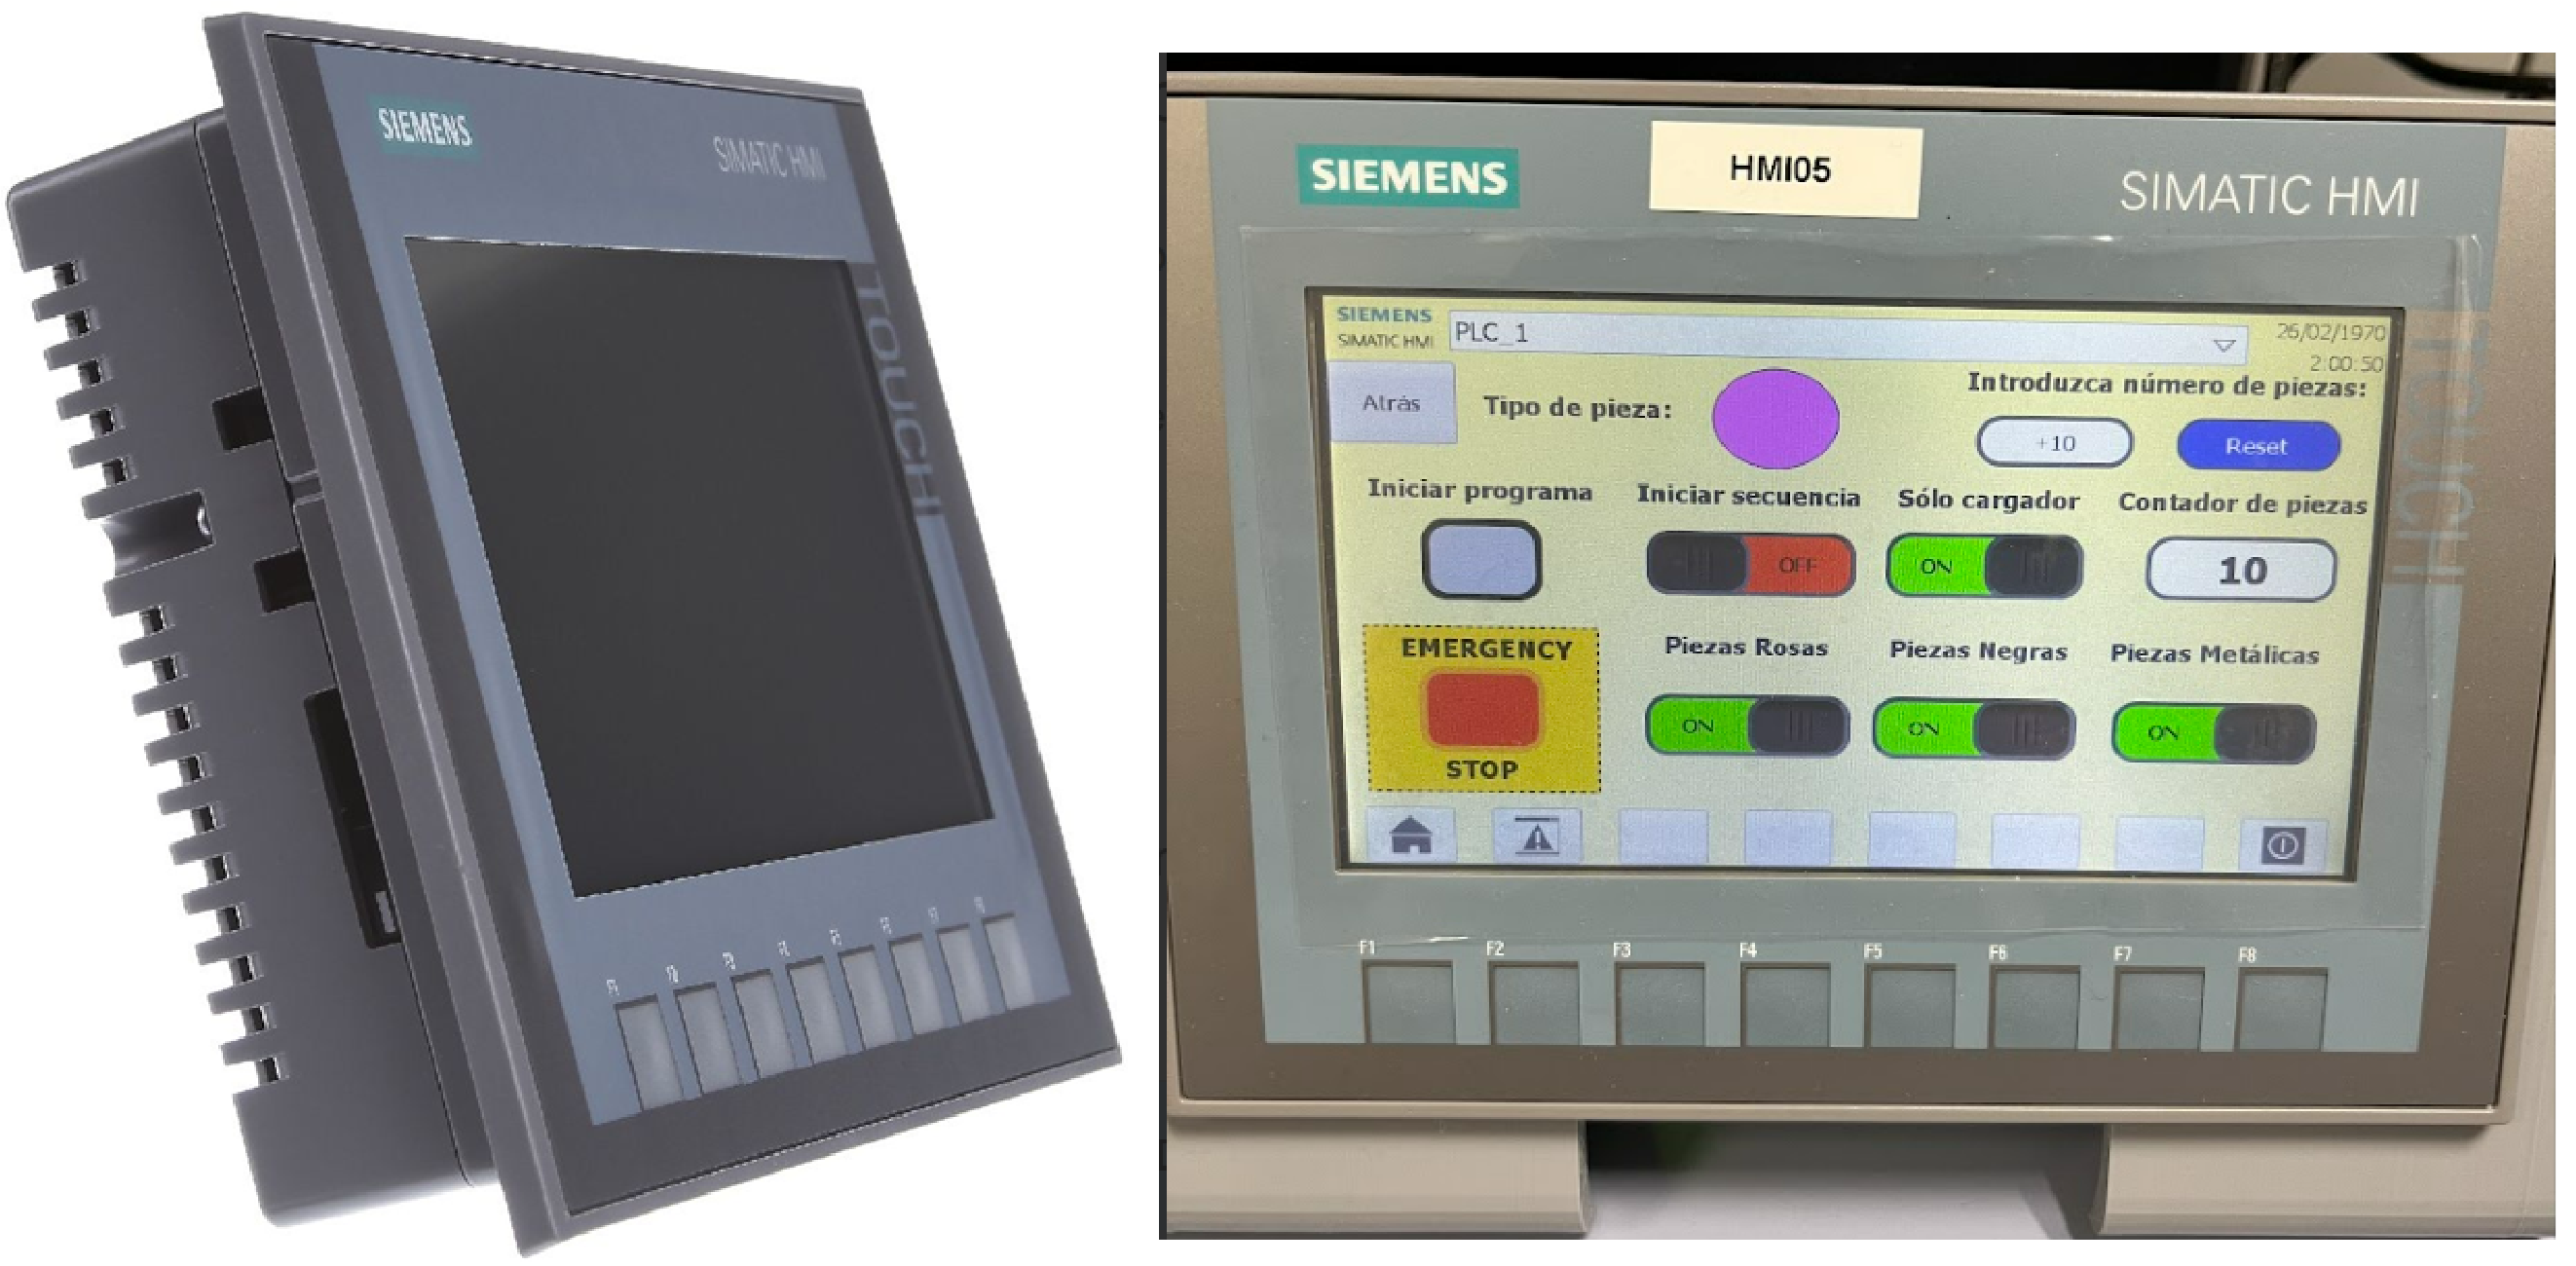
\includegraphics[width=15cm]{figs/HMI_cap_3}
  \end{center}
  \caption{\centering SIMATIC HMI KTP700 Basic PN.}
  \label{fig:HMI_cap_3}
\end{figure} 

El KTP700 Basic PN dispone de una interfaz USB que permite conectar dispositivos periféricos como ratones, teclados o memorias USB para la transferencia de recetas, actualizaciones de firmware o copias de seguridad de datos de usuario \cite{HMI_KTP}. Además, este HMI admite la configuración y programación a través del entorno de desarrollo TIA Portal (Totally Integrated Automation) con WinCC Basic, lo que asegura una integración coherente y eficiente con el resto de componentes del sistema de automatización \cite{HMI_KTP}.

En cuanto a su diseño físico, el dispositivo tiene unas dimensiones compactas de 214 × 158 × 39 mm y está pensado para montaje en panel \cite{HMI_KTP}. Cuenta con una protección frontal IP65, lo que le confiere resistencia frente a polvo y chorros de agua, haciéndolo apto para condiciones industriales exigentes \cite{HMI_KTP}. También incluye funciones como alarmas, tendencias, gestión de recetas y multilenguaje, lo que lo convierte en una solución versátil para aplicaciones industriales básicas.

\section{TIA Portal}
\label{sec:tia_portal}

TIA Portal (Totally Integrated Automation Portal) es una plataforma de ingeniería desarrollada por Siemens que integra en un único entorno todas las herramientas necesarias para la configuración, programación, supervisión y mantenimiento de sistemas de automatización industrial. Fue diseñado con el objetivo de unificar y simplificar la ingeniería de proyectos, mejorando la eficiencia en el desarrollo, la puesta en marcha y la operación de sistemas de control.

\begin{figure} [h!]
  \begin{center}
    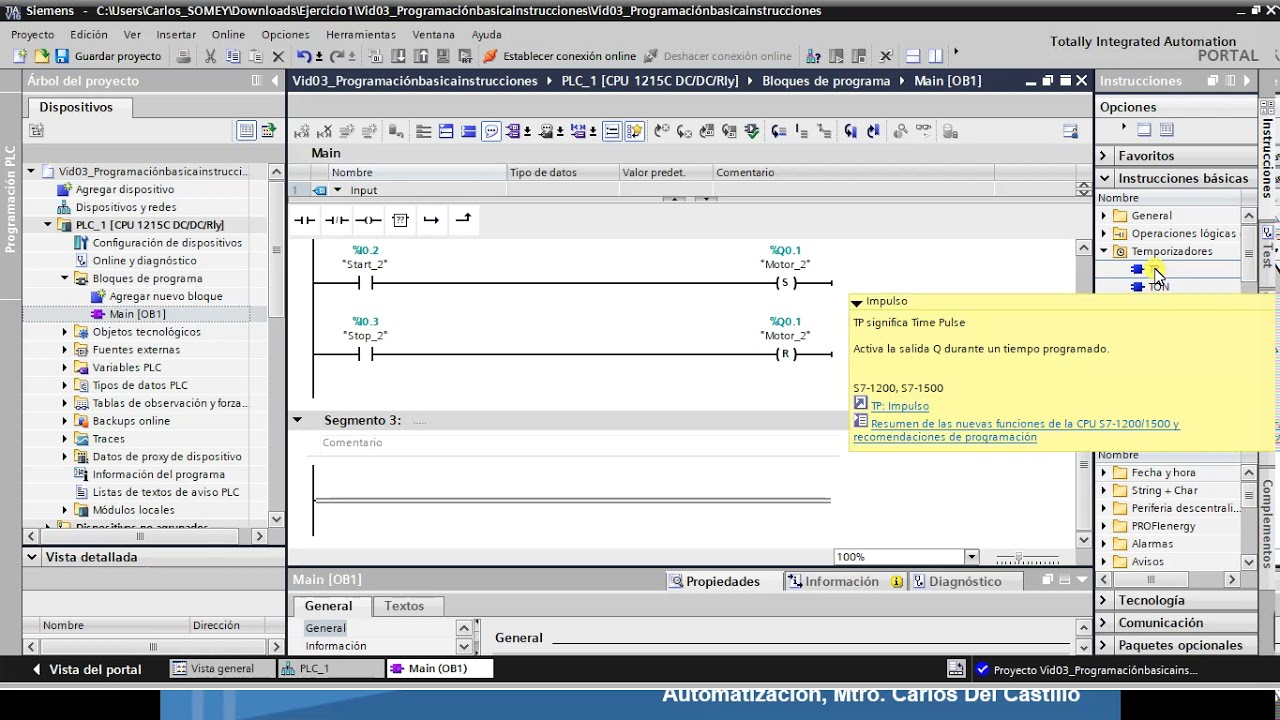
\includegraphics[width=14cm]{figs/TIA_portal}
  \end{center}
  \caption{\centering Captura de pantalla de la aplicación TIA Portal.}
  \label{fig:TIA_portal}
\end{figure} 

Esta plataforma permite trabajar de forma integrada con controladores PLC, interfaces HMI, sistemas SCADA, variadores de velocidad, dispositivos de seguridad y redes industriales, todo desde una única interfaz \cite{TIA_portal}. El entorno TIA Portal combina software como STEP 7 (para programación de PLC), WinCC (para interfaces HMI y SCADA), Startdrive (para variadores SINAMICS), Safety Advanced (para funciones de seguridad) y Energy Suite (para gestión energética) \cite{TIA_portal}.

En este proyecto se ha utilizado la versión \textbf{TIA Portal V16}, la cual permitedividir los proyectos en unidades de software independientes, permitiendo una programación modular con interfaces definidas \cite{TIA_portal}. Esto facilita la colaboración entre varios ingenieros, mejora la reutilización de código y simplifica la gestión de proyectos complejos.

En cuanto a la programación de PLCs, TIA Portal V16 ofrece soporte completo para los controladores SIMATIC S7-1200, S7-1500, S7-300 y S7-400, así como para soluciones de seguridad integradas mediante STEP 7 Safety \cite{TIA_portal}. La integración con WinCC permite el diseño y configuración de interfaces HMI.

La plataforma también incluye herramientas de simulación como PLCSIM y HMISIM, que permiten probar y validar la lógica de control y las interfaces HMI sin necesidad de hardware físico \cite{TIA_portal}. Esto reduce los tiempos de desarrollo y facilita la detección temprana de errores. Además, la compatibilidad con estándares abiertos y protocolos de comunicación como PROFINET, OPC UA y Modbus garantiza una integración fluida con otros sistemas y dispositivos en entornos de automatización industrial \cite{TIA_portal}.

\section{Cobot UR5e}
\label{sec:ur5e}

El UR5e es un brazo robótico colaborativo de seis ejes desarrollado por Universal Robots, diseñado para automatizar tareas industriales de forma segura y eficiente. Con una capacidad de carga útil de hasta 5 kg y un alcance de 850 mm, el UR5e es especialmente adecuado para aplicaciones que requieren precisión y flexibilidad, como ensamblaje, manipulación de materiales, soldadura ligera y pruebas de calidad \cite{UR5e}.

\begin{figure} [h!]
  \begin{center}
    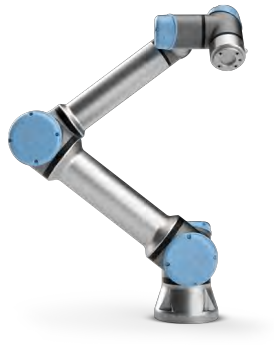
\includegraphics[width=8.4cm]{figs/UR5e}
  \end{center}
  \caption{\centering Robot UR5e de Universal Robots. \cite{UR5e}}
  \label{fig:UR5e}
\end{figure} 

Una de las características distintivas del UR5e es su diseño colaborativo, que permite su integración en entornos donde comparte espacio con operadores humanos sin necesidad de barreras de seguridad, siempre que se realice una evaluación de riesgos adecuada \cite{UR5e}. Esto es posible gracias a sus sensores de fuerza y par integrados, que detectan contactos inesperados y detienen el movimiento del robot para evitar lesiones o daños \cite{UR5e}.

El UR5e se controla mediante el software PolyScope, una interfaz intuitiva que se opera a través de un panel de enseñanza con pantalla táctil. PolyScope permite programar el robot de manera sencilla, incluso sin experiencia previa en programación, mediante la guía manual del brazo para enseñar posiciones y trayectorias \cite{UR5e}. Para usuarios avanzados, también se ofrece la posibilidad de programar utilizando el lenguaje URScript, lo que proporciona un mayor control y flexibilidad en aplicaciones complejas.

Su diseño ligero, con un peso total de aproximadamente 20,6 kg, permite montarlo en diversas orientaciones y ubicaciones, adaptándose a diferentes necesidades de producción \cite{UR5e}. Además, el UR5e es compatible con una amplia gama de accesorios y herramientas a través del ecosistema UR+, que ofrece soluciones certificadas para tareas específicas, como pinzas, cámaras y sensores adicionales \cite{UR5e}. 

\begin{figure} [h!]
  \begin{center}
    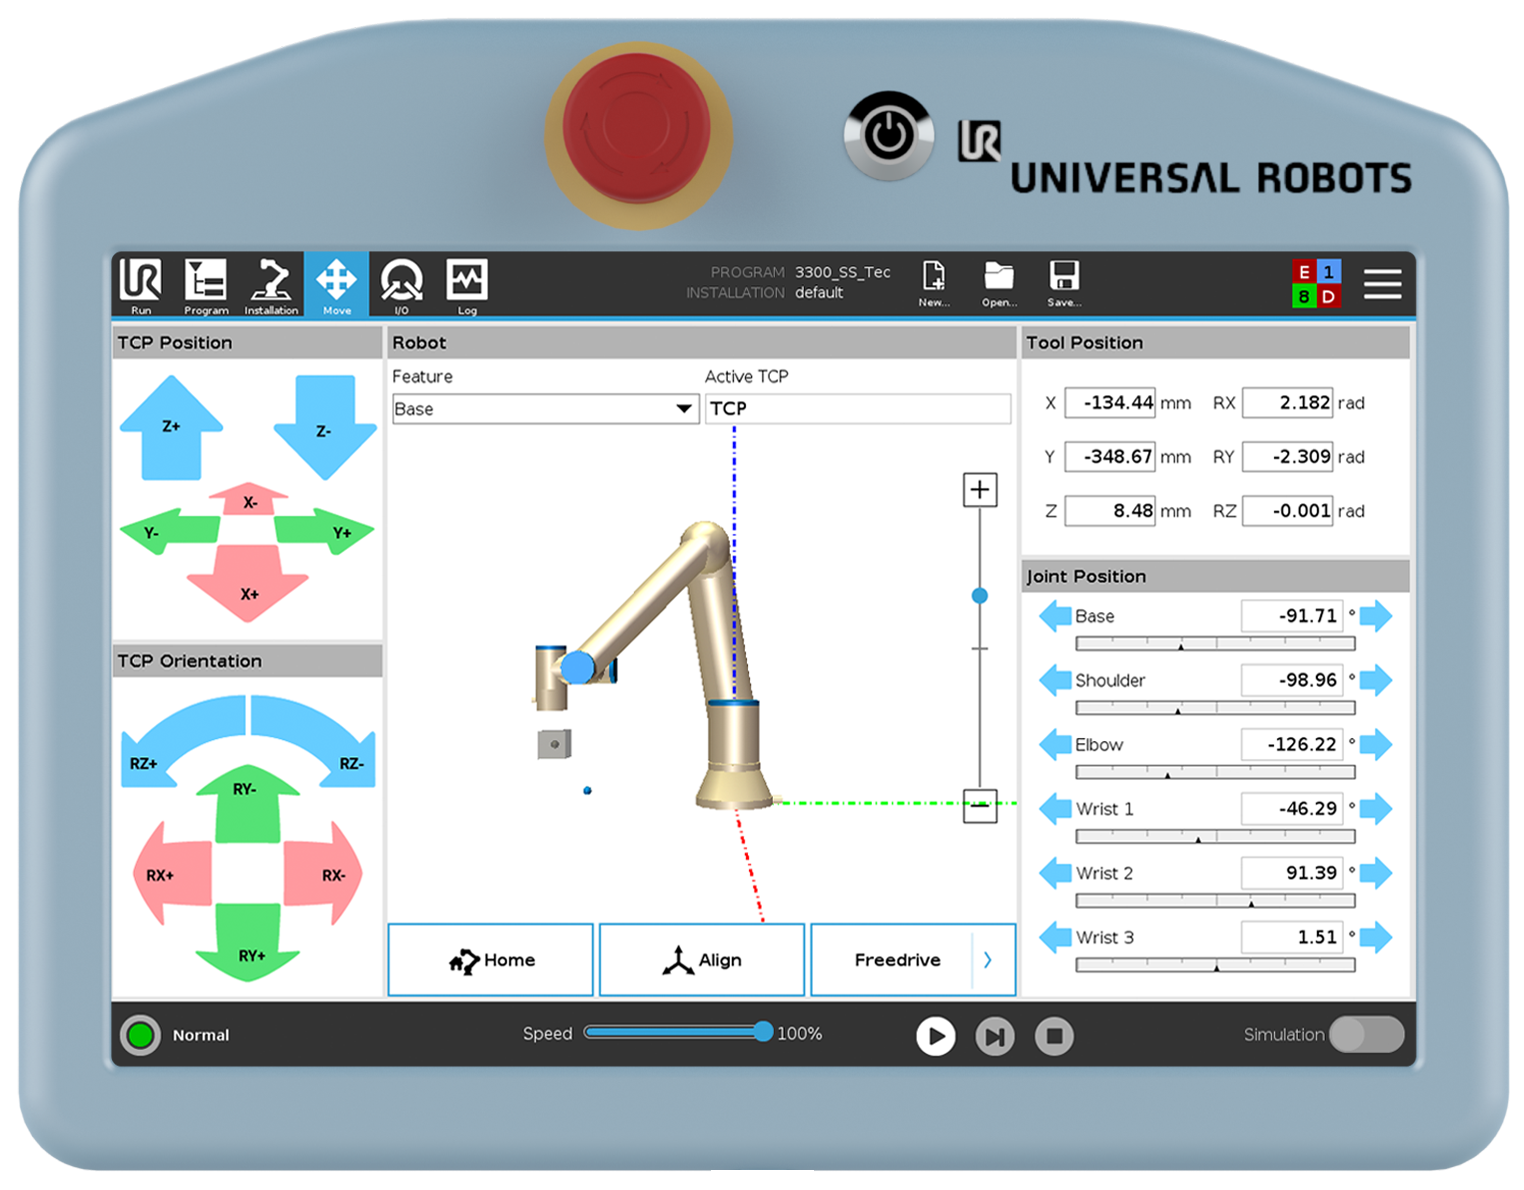
\includegraphics[width=10.5cm]{figs/PolyScope}
  \end{center}
  \caption{\centering Pantalla táctil PolyScope. \cite{PloyScope_img}}
  \label{fig:PolyScope}
\end{figure} 

\section{Switch ethernet industrial}
\label{sec:switch_industrial}

En el sistema se ha utilizado el modelo 6GK5005-0GA10-1AB2 de Siemens, un switch Ethernet industrial de tipo no gestionado perteneciente a la gama SCALANCE XB005\footnote{SCALANCE XB-000 unmanaged. (2025).\url{https://mall.industry.siemens.com/mall/es/es/Catalog/Product/6GK5005-0BA00-1AB2}} \cite{switch_industrial}. Este dispositivo proporciona cinco puertos RJ-45 con soporte para velocidades de 10/100/1000 Mbit/s, lo cual lo hace adecuado para redes industriales donde se requiere una comunicación eficiente y estable entre distintos equipos, como controladores, paneles HMI o dispositivos de supervisión \cite{switch_industrial}.  \\

Su diseño está orientado a aplicaciones industriales, funciona con una tensión de alimentación de 24 V DC y presenta un consumo reducido, lo cual es beneficioso en términos de eficiencia energética \cite{switch_industrial}. A pesar de no ser gestionable, incorpora indicadores LED que permiten supervisar el estado de los enlaces y la actividad de red en tiempo real \cite{switch_industrial}. Además, ofrece compatibilidad con PROFINET, siendo una solución adecuada para pequeñas topologías dentro de entornos industriales controlados \cite{switch_industrial}. \\

\begin{figure} [h!]
  \begin{center}
    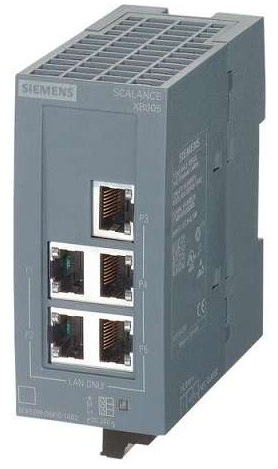
\includegraphics[width=5cm]{figs/switch_industrial}
  \end{center}
  \caption{\centering Switch industrial 6GK5005-0GA10-1AB2 de Siemens \cite{switch_industrial}}
  \label{fig:switch_industrial}
\end{figure}

